%% ****** Start of file aiptemplate.tex ****** %
%%
%%   This file is part of the files in the distribution of AIP substyles for REVTeX4.
%%   Version 4.1 of 9 October 2009.
%%
%
% This is a template for producing documents for use with 
% the REVTEX 4.1 document class and the AIP substyles.
% 
% Copy this file to another name and then work on that file.
% That way, you always have this original template file to use.

\documentclass[aip,rsi]{revtex4-1}
\usepackage{graphicx}
%\documentclass[aip,reprint]{revtex4-1}

%\draft % marks overfull lines with a black rule on the right

\begin{document}

% Use the \preprint command to place your local institutional report number 
% on the title page in preprint mode.
% Multiple \preprint commands are allowed.
%\preprint{}

\title{High Resolution Time of Flight Mass Spectrometer for Measuring Products in Heterogenous Catalysis in Higly Sensitive Microreactors} %Title of paper

% repeat the \author .. \affiliation  etc. as needed
% \email, \thanks, \homepage, \altaffiliation all apply to the current author.
% Explanatory text should go in the []'s, 
% actual e-mail address or url should go in the {}'s for \email and \homepage.
% Please use the appropriate macro for the type of information

% \affiliation command applies to all authors since the last \affiliation command. 
% The \affiliation command should follow the other information.

\author{T. Andersen}
\author{R. Jensen}
\author{....}
\affiliation{CINF, Department of Physics...}
\author{O. Hansen}
\affiliation{CINF, Department of Micro- and Nanotechnology}
\author{I. Chorkendorff}
\email[]{ibchork@fysik.dtu.dk}
\affiliation{CINF, Department of Physics...}
%\homepage[]{Your web page}
%\thanks{}
%\altaffiliation{}
%\affiliation{}

% Collaboration name, if desired (requires use of superscriptaddress option in \documentclass). 
% \noaffiliation is required (may also be used with the \author command).
%\collaboration{}
%\noaffiliation

\date{\today}

\begin{abstract}
We demonstrate that high resolution time of flight mass spectrometry can be successfully applied to detect gas-phase product in hetrogeneous catalysis. Combining the instrument with the highly sensitive microreactors opens the possibility to measure on system that are otherwise difficult due to ....
\end{abstract}

\pacs{}% insert suggested PACS numbers in braces on next line

\maketitle %\maketitle must follow title, authors, abstract and \pacs

% Body of paper goes here. Use proper sectioning commands. 
% References should be done using the \cite, \ref, and \label commands
\section{Introduction}
In heterogeneous catalysis the optimization and development of equipment is important both to minimize the cost of equipment but also to be able to study complicated systems. As a platform for testing heterogeneous catalysts microfabricated reactors or microreactors have been found suitable due to both the high surface-to-volume ratio, the fast temperature response and minimization of thermal and concentration gradients. Such a platform have among other places been developed in our department \cite{Henriksen2009}. However, a suitable reactor platform is only part of the task. Typically, quadrupole mass spectrometers (QMSs) are used in low pressure regimes to analyze gas composition while gas chromatographs are used for high pressure measurements. The QMS, however, suffer from a low mass resolution ($\Delta$m/m$\sim$200) which makes analysis of complicated spectra difficult and cumbersome and a low mass range (typically up to $\sim$500\,amu). Furthermore, QMSs are typically operated by logging a single (or a few) masses as a function of time to increase the time resolution. This in turn is on the expense of being unable to acquire full mass spectra continuously. Something negative about chromatographs... As an alternative time of flight mass spectrometers (TOF-MS) offer both high mass resolution ($\Delta$m/m$>$400) and fast acquisition of full mass spectra ($>$1\,Hz) along with mass range only limited by the detector. For a typical microchannel plate (MCP) a mass range of (0--5000\,amu) can be obatined Until now, to our knowlegde, the testing of catalysts in a microreactor with subsequent gas analysis by a TOF-MS have not been demonstrated. Here we desribe a microreactor and TOF-MS system which combines the high sensitivity of microreactors and the high mass resolution TOF-MSs for use in heterogeneous catalysis.

\section{System design}
The complete system enables high sensitivity reactivity measurements of the catalyst under investigation combined with high resolution mass spectrometry. The catalyst under investigation is deposited in a microreactor from where the products are detected with time of flight mass spectrometry. A schematic of the entire setup is shown in Figure \ref{fig:TOF_microreactor}
\begin{figure}
 \includegraphics[width=14cm]{TOF_microreactor.png}%
 \caption{Schematic of the total system (not to scale)\label{fig:TOF_microreactor}}%
\end{figure}
Three setup consists of three main components. The microreactor where the catalyst under investigation is deposited, an ionization source which ionizes the gas from the microreactor and the TOF equipment used for gas analysis. 

\subsection{Microreactor and gas handling}

\subsubsection{The microreactor platform}
Catalysts testing were performed in a microreactor platform \cite{Henriksen2009}. The microreactors are fabricated in silicon and measures 20x15\,mm. The reactor consists of two gas inlets, a gas outlet, a reactor volume and a capillary used for probing the gas from the reactor volume. The reactor volume is 3\,$\mu$m deep and 1 cm in diameter resulting in a 240\,nL volume. The two gas inlets are combined on the chip where the inlet gases mix by diffusion. The capillary is designed such that approximately $3\cdot10^{14}$\,molecules$\cdot$s$^{-1}$ is probed from the reactor volume. Any surplus of gas from the two inlets that does not enter the reactor volume is directed through the outlet into a turbo pump. The design ensures that all molecules entering the reactor volume hence exposed to the catalyst under investigation is detected giving the system high sensitivity.

The microreactor is heated by joule heating of a 50 nm platinum strip evaporated through a shadow mask on the backside of the chip. The heating element is contacted by two pogo pins which is connected to a power supply. Additionally, two extra contacts are placed on the chip which facilitates 4 wire measurement of the resistance of the heating element. The heating strip is hence used as a resistance temperature detector (RTD) to monitor the temperature of the chip. At the current configuration temperatures from room temperature to approximately 450\,$^{\circ}$C can be reached.


\subsubsection{Gas handling}
The two gas inlets on the microreactor chip is connected to a gas handling system. A total of 6 gases with accompanying flow controllers are used to control the inlet gas. Currently, the system is configured in a 4+2 setup where 4 gases are connected to the one inlet and to gases on the other inlet. All valves and flow controllers are interfaced to computer enabling remote control of the system and the possibility to run experiments over several days without human intervention.

\subsection{Time of flight}
The time of flight equipment used for detection of gas molecules flowed through the capillary of the microreactor is designed as an orthogonal mass spectrometer. Ionized ions enter the source through a series of Einzel lenses used for focusing the beam minimizing divergence. In the source they are pushed into the flight tube by an the initial push voltage, V$_p$. The ions are further accelerated from ground potential to the liner potential, V$_L$, which is the drift voltage of the flight tube. At the end of the flight tube a reflectron is installed which have two primary purposes. The effective drift length is increased hence increasing resolution of the equipment. The reflectron also works as a focusing lens compensating for any initial velocity dispersion of the ions, i.e. ions with an initial higher velocity will have an increased flight length compared to slower ions. The microchannel plate (MCP) used for detection is placed in the focal point of the reflectron giving maximum compensation for initial velocity dispersion. The theoretical resolution of the equipment is $\Delta$m/m$\sim$4000.

\begin{figure}
 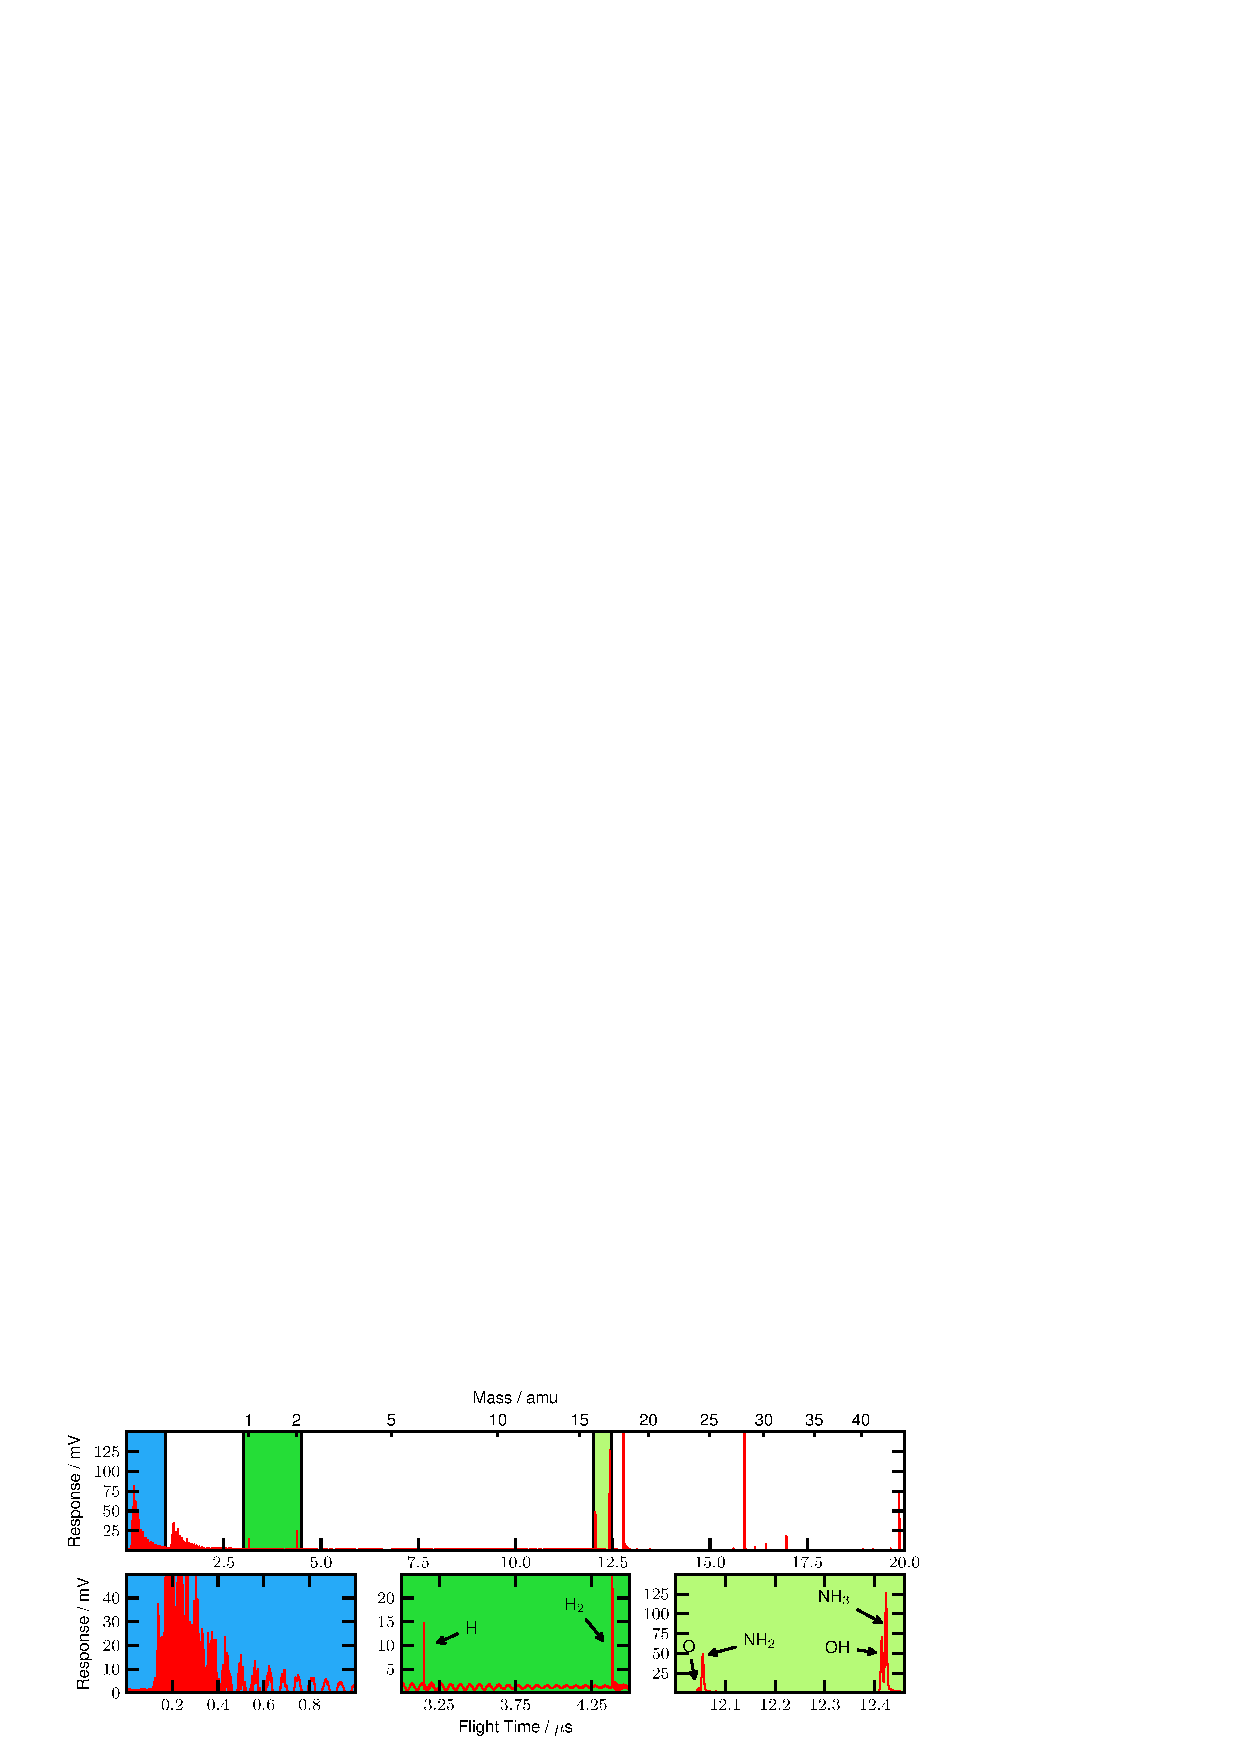
\includegraphics[width=14cm]{untreated_data.png}%
 \caption{Untreated data from the TOF-MS showing methanol and air.\label{fig:untreated_data}}%
\end{figure}


\subsubsection{Ionization of gas}
As ionization source of the gas flow from the microreactor capillary an modified nude UHV Bayard-Alpert ion gauge is used. Approximately 3\,A is run through the filament resulting in approximately 10\,mA emission current. The grid is biased approximately 40\,V negative compared to the filament to accelerate electrons emitted from the filament towards the grid. Contrary to standard operation of a ion gauge the collector in the center of the grid is short-circuited to grid to ensure homogeneous field distribution within the grid. To allow ionized ions to escape from the grid the lid of the grid have been removed. Using this configuration approximately half of the ionized ions are expected to leave the ionization gauge. The entire construction is placed in a nozzle which is differentially pumped. Large amounts of gases can hence be dosed locally around the ion gauge while still maintaining a low pressure in the source region of the TOF. The nozzle is essential in the setup to avoid high pressure in the source region resulting in a increase in dead counts on the MCP thus decreasing the noise to signal ratio of the recorded signal.

\subsubsection{Data treatment}
\begin{figure}
 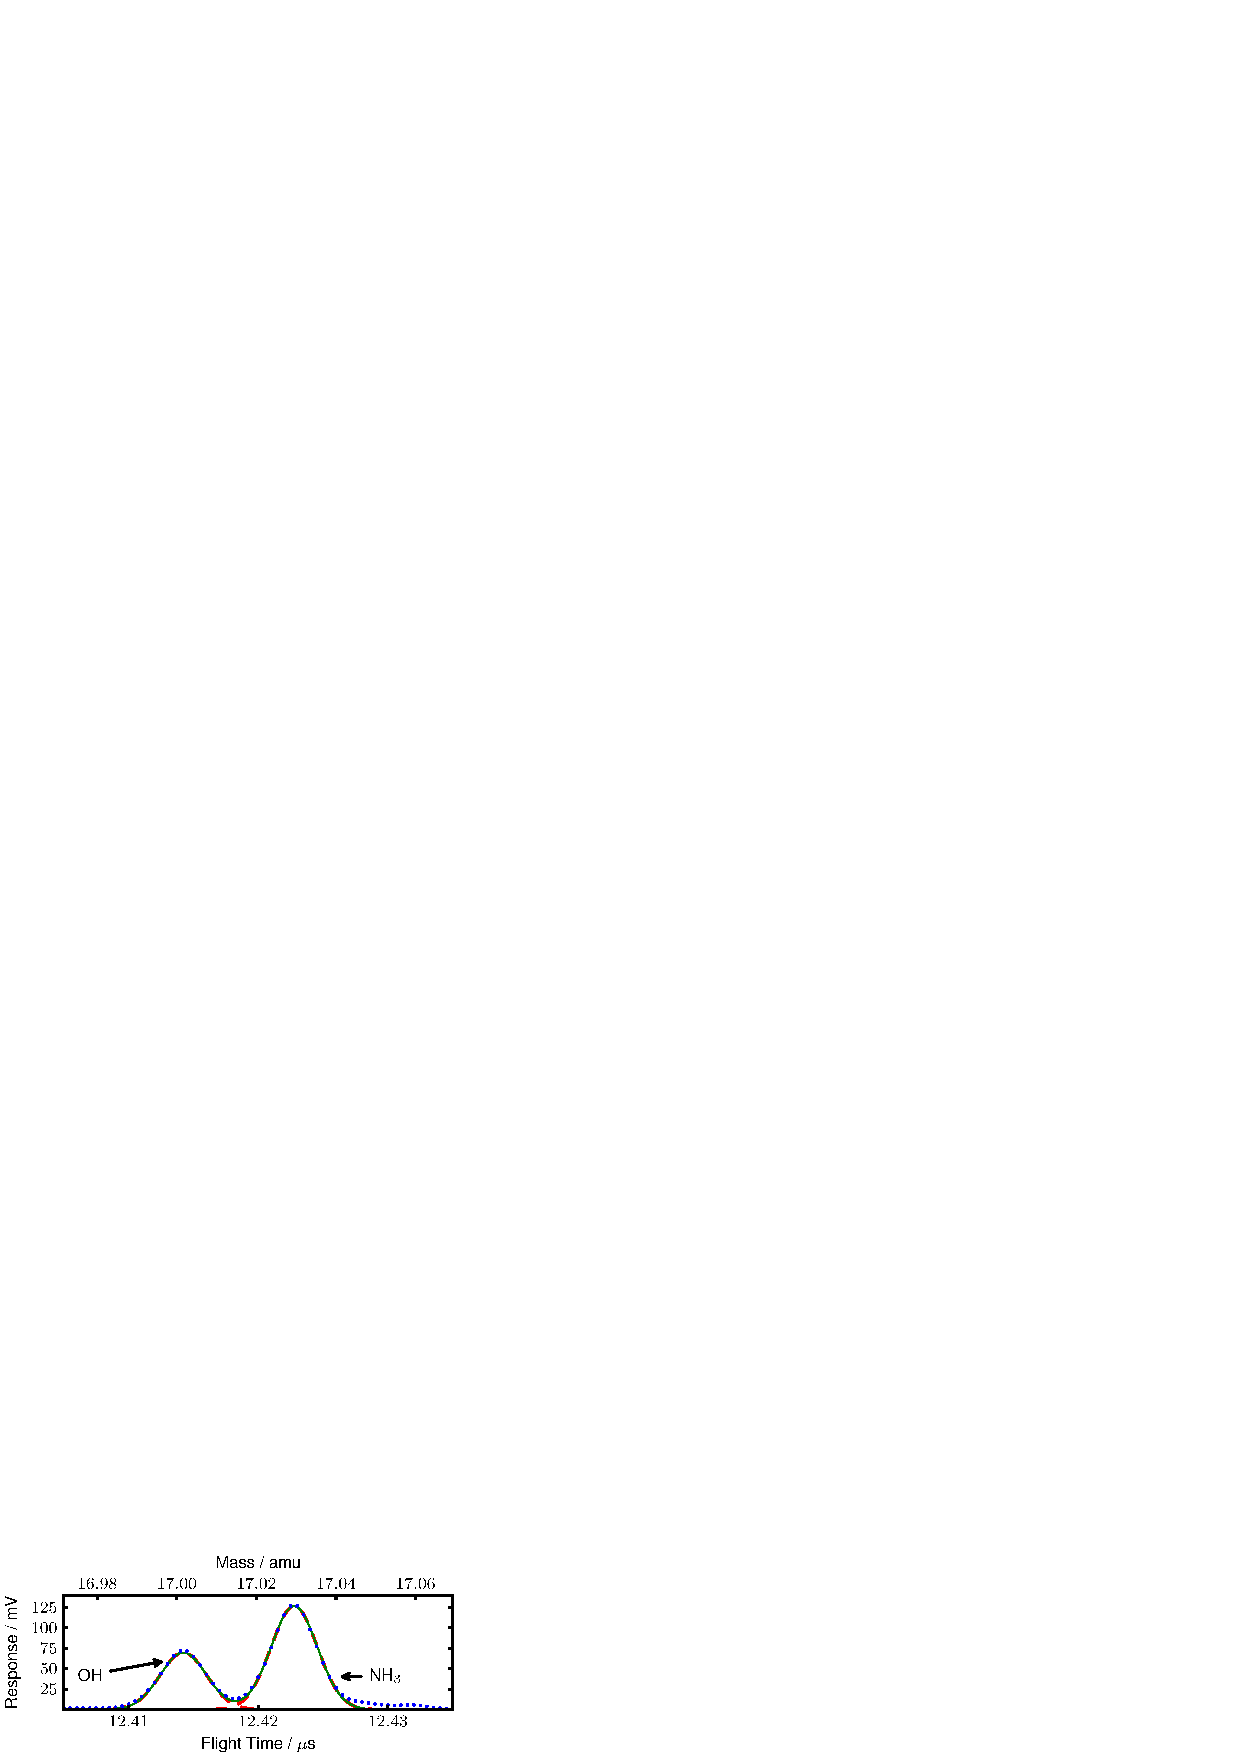
\includegraphics[width=14cm]{ammonia_OH_gauss_fit.png}%
 \caption{Example of Gaussion fit to a double peak. Each gaussion yields the area of the respective component.\label{fig:gaussian_fit}}%
\end{figure}


\section{Test system}
Ammonia oxidation


\section{Summary}

\section{Acknowledgements}

% If in two-column mode, this environment will change to single-column format so that long equations can be displayed. 
% Use only when necessary.
%\begin{widetext}
%$$\mbox{put long equation here}$$
%\end{widetext}

% Figures should be put into the text as floats. 
% Use the graphics or graphicx packages (distributed with LaTeX2e).
% See the LaTeX Graphics Companion by Michel Goosens, Sebastian Rahtz, and Frank Mittelbach for examples. 
%
% Here is an example of the general form of a figure:
% Fill in the caption in the braces of the \caption{} command. 
% Put the label that you will use with \ref{} command in the braces of the \label{} command.
%
% \begin{figure}
% \includegraphics{}%
% \caption{\label{}}%
% \end{figure}

% Tables may be be put in the text as floats.
% Here is an example of the general form of a table:
% Fill in the caption in the braces of the \caption{} command. Put the label
% that you will use with \ref{} command in the braces of the \label{} command.
% Insert the column specifiers (l, r, c, d, etc.) in the empty braces of the
% \begin{tabular}{} command.
%
% \begin{table}
% \caption{\label{} }
% \begin{tabular}{}
% \end{tabular}
% \end{table}

% If you have acknowledgments, this puts in the proper section head.
%\begin{acknowledgments}
% Put your acknowledgments here.
%\end{acknowledgments}

% Create the reference section using BibTeX:
\bibliographystyle{abbrv}
%\bibliographystyle{alpha}
%\bibliographystyle{plain}
\bibliography{literature}

\end{document}
%
% ****** End of file aiptemplate.tex ******
